\documentclass[border=10pt]{standalone}
\usepackage[T1]{fontenc}
\usepackage{times}
\usepackage{tikz}
\usetikzlibrary{arrows.meta}

\begin{document}
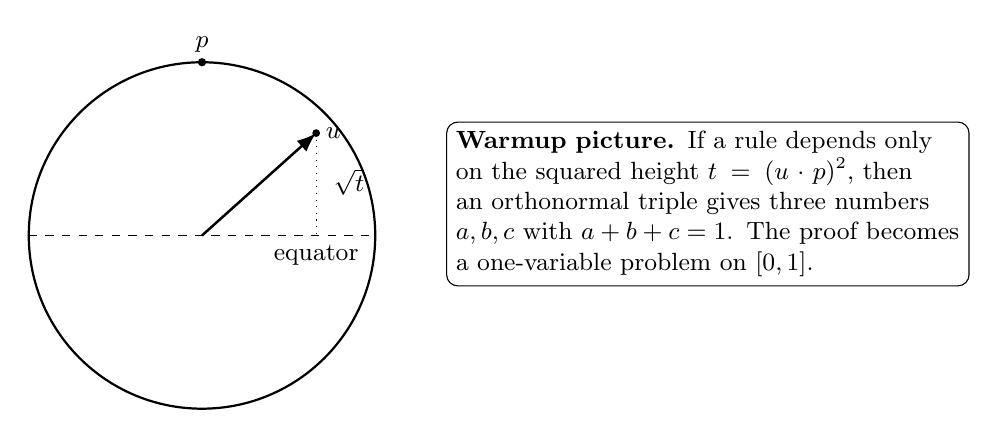
\begin{tikzpicture}[>=Latex, font=\small]
\draw[line width=0.8pt] (0,0) circle (2.2);
\draw[dashed] (-2.2,0) -- (2.2,0);
\fill (0,2.2) circle (1.5pt);
\node[above] at (0,2.2) {$p$};
\fill (1.45,1.3) circle (1.4pt);
\node[right] at (1.45,1.3) {$u$};
\draw[->, line width=0.9pt] (0,0) -- (1.45,1.3);
\draw[dotted] (1.45,1.3) -- (1.45,0);
\node[below] at (1.45,0) {equator};
\node[right] at (1.55,0.68) {$\sqrt{t}$};

\node[draw, rounded corners=4pt, align=left, fill=white, text width=6.4cm, anchor=west]
at (3.1,0.4) {%
\textbf{Warmup picture.}
If a rule depends only on the squared height $t=(u\cdot p)^2$, then an orthonormal triple gives three numbers $a,b,c$ with $a+b+c=1$. The proof becomes a one-variable problem on $[0,1]$.};
\end{tikzpicture}
\end{document}
